\begin{figure}[htbp]
  \begin{tabular}{cc}
    \begin{minipage}{0.5\hsize}
      \centering
      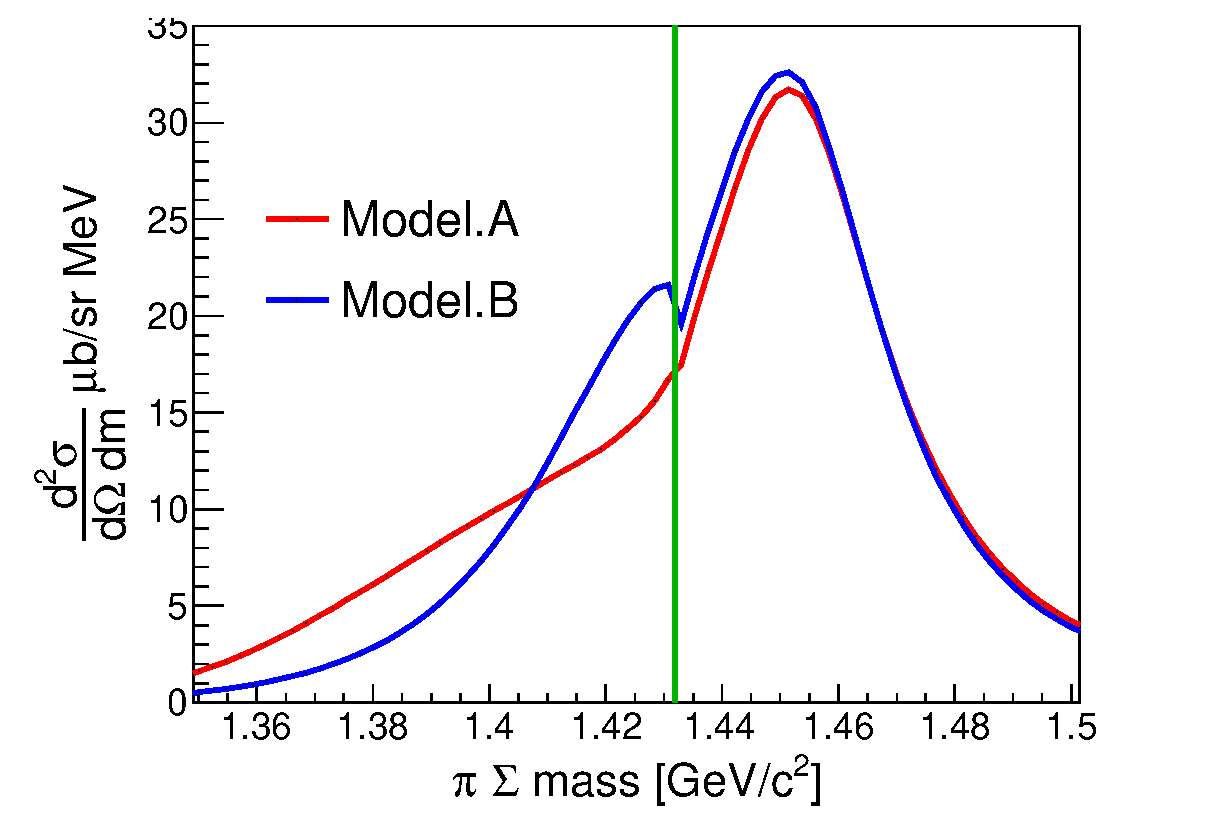
\includegraphics[width=6.0cm]{../pic/Dron/discussion/DCC_pimSp.eps}
    \end{minipage}
    
    \begin{minipage}{0.5\hsize}
      \centering
      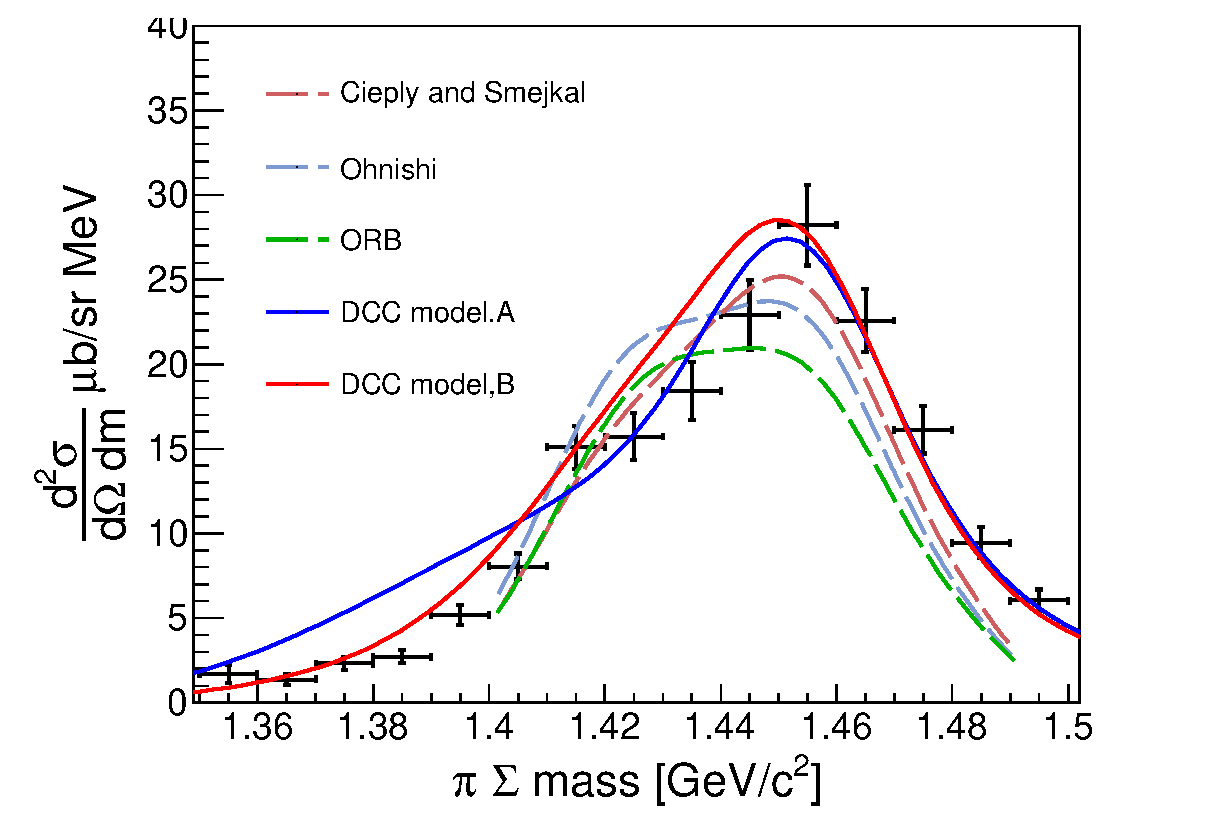
\includegraphics[width=6.0cm]{../pic/Dron/discussion/miyagawa_pimSp.eps}
    \end{minipage}
  \end{tabular}

  \begin{tabular}{cc}
    \begin{minipage}{0.5\hsize}
      \centering
      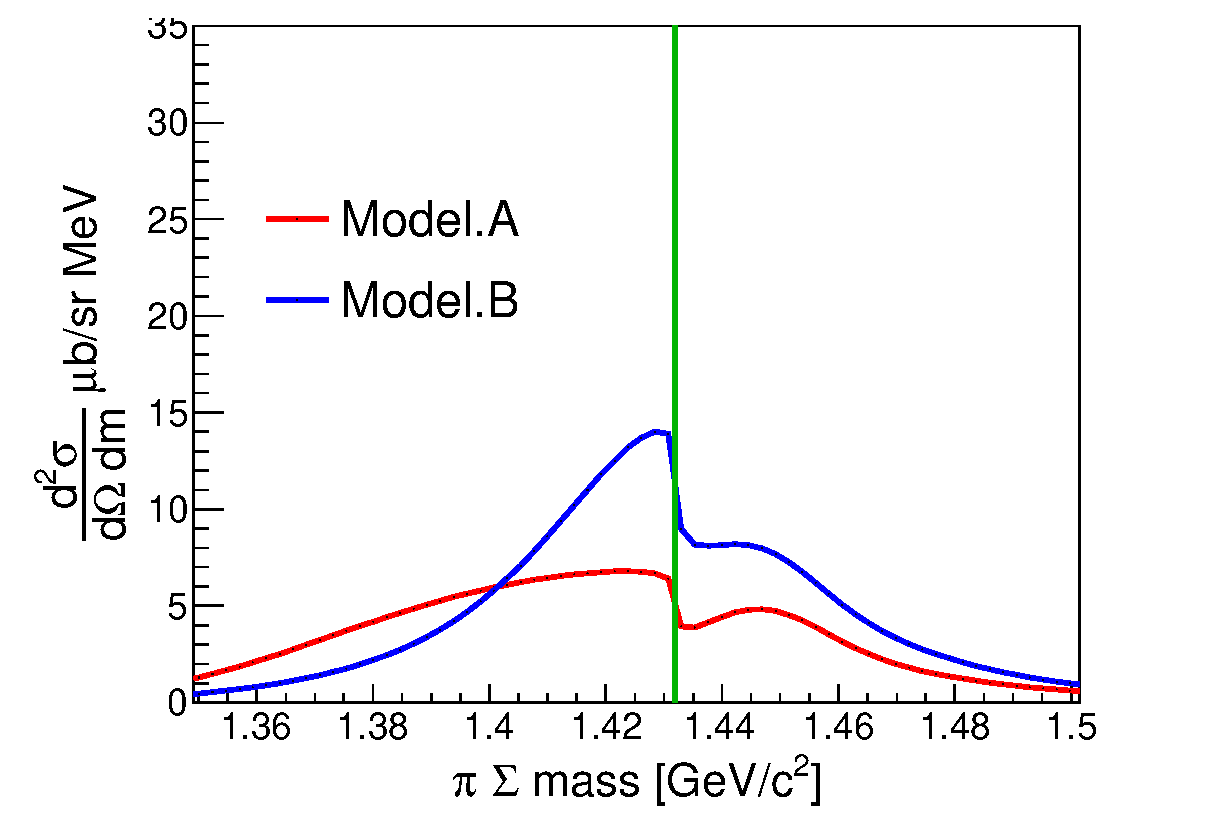
\includegraphics[width=6.0cm]{../pic/Dron/discussion/DCC_pipSm.eps}
    \end{minipage}
    
    \begin{minipage}{0.5\hsize}
      \centering
      \includegraphics[width=6.0cm]{../pic/Dron/discussion/miyagawa_pipSm.eps}
    \end{minipage}
  \end{tabular}

  \begin{tabular}{cc}
    \begin{minipage}{0.5\hsize}
      \centering
      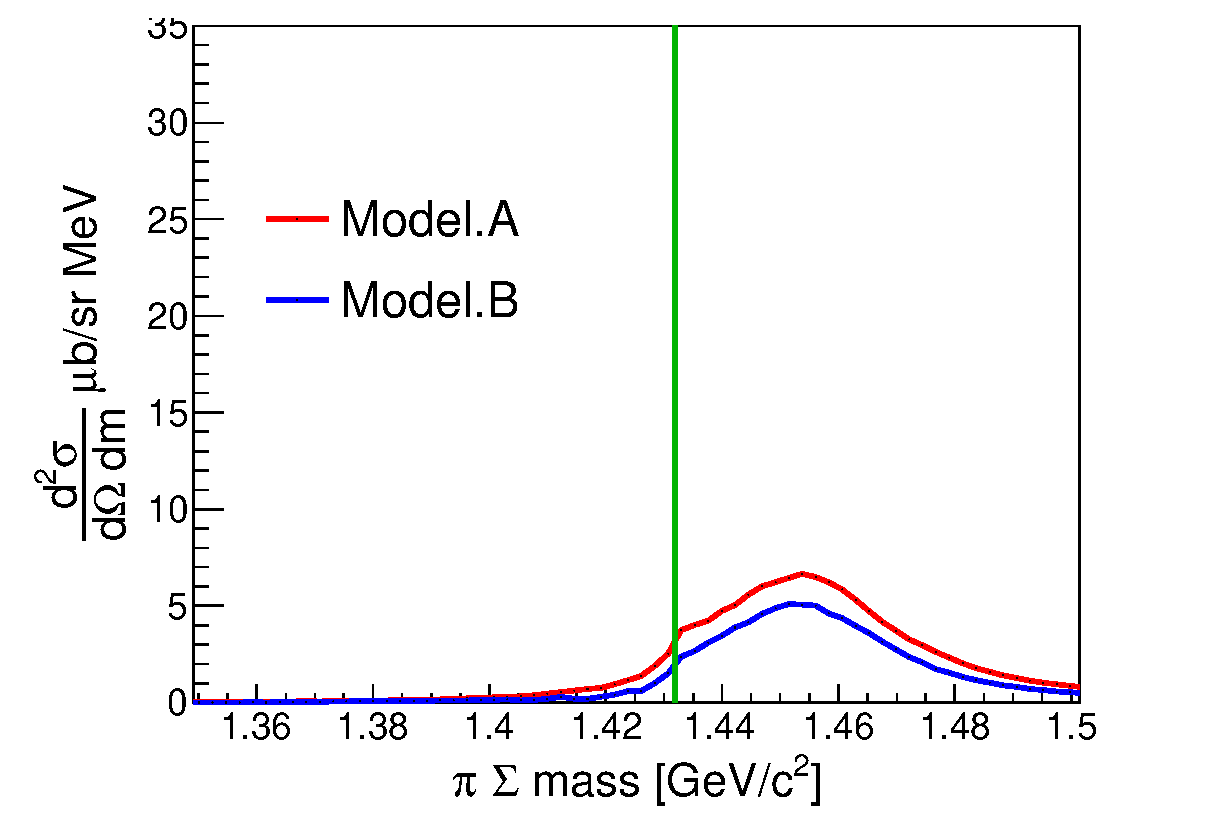
\includegraphics[width=6.0cm]{../pic/Dron/discussion/DCC_pimS0.eps}
    \end{minipage}
    
    \begin{minipage}{0.5\hsize}
      \centering
      \includegraphics[width=6.0cm]{../pic/Dron/discussion/miyagawa_pimS0.eps}
    \end{minipage}
  \end{tabular}
  
  \caption{
    This figure shows a comparison of our obtained spectra with predictions from theoretical calculations.
    The top, middle, and bottom figures represent $\pi^-\Sigma^+$, $\pi^+\Sigma^-$, and $\pi^-\Sigma^0$, respectively.
    The right figure shows the spectrum predicted by the DCC model, and the left figure shows the spectrum predicted by the calculation of Miyagawa et al.
    The spectra predicted by theoretical calculations are convoluted with our detector resolution.
  }
  \label{fig:comp_theoretical_calc}
\end{figure}
